\section{Mathematical Foundations of Cosmochrony — Dynamics, Stability, and Analytical Solutions}
  \label{sec:appendix-math}

  This appendix provides a rigorous mathematical formulation of the $\chi$-field
  dynamics underlying the Cosmochrony framework.
  Its purpose is not to introduce new physical assumptions, but to support the
  effective descriptions developed in the main text by establishing the internal
  consistency, stability properties, and analytical structure of the underlying
  field equations.

  In particular, this appendix presents:
  \begin{itemize}
    \item an effective Lagrangian formulation and its hydrodynamic limit
    (Section~\ref{subsec:hydrodynamic-limit}),
    \item stability analyses of the $\chi$ field under perturbations
    (Section~\ref{subsec:stability-analysis}),
    \item analytical solutions in homogeneous, spherically symmetric, and planar
    regimes (Section~\ref{subsec:analytical-solutions}),
    \item and the relational foundation of emergent geometric descriptions
    (Section~\ref{app:relational_formulation}).
  \end{itemize}

  All results are derived from the fundamental postulates of Cosmochrony
  (Section~\ref{subsec:geometric-action}) without assuming a pre-existing spacetime
  metric or background geometry.
  Geometric notions appearing in this appendix should therefore be understood as
  effective and coarse-grained representations of the underlying $\chi$ dynamics,
  consistent with the interpretative framework developed in Appendix~\cite{sec:appendix-technical}.

  No additional physical assumptions are introduced in this appendix; all results
  follow from reformulations, approximations, or limiting regimes of the same
  underlying $\chi$ dynamics discussed in the main text.

  Several structures derived here—such as relaxation bounds, stability spectra, and
  effective coupling scalings—provide the mathematical basis for the phenomenological
  signatures discussed in Section~\ref{sec:testable-predictions-and-observational-signatures},
  without constituting independent predictive postulates.

  \subsection{Effective Lagrangian Description as a Hydrodynamic Limit}
  \label{subsec:hydrodynamic-limit}

  \noindent\emph{The purpose of this subsection is not to introduce any additional
fundamental structure into Cosmochrony, but to provide an effective hydrodynamic
tool for connecting the relational $\chi$ framework to standard geometric
formulations in regimes where a spacetime description becomes operationally
meaningful.}

  \subsubsection*{From Relational Dynamics to an Effective Continuum Description}

    At the fundamental level, Cosmochrony is defined without reference to any
    pre-existing spacetime manifold or metric structure.
    The dynamics of the $\chi$ field are relational and are specified directly in
    terms of local relaxation rules and coupling relations between configurations
    (Section~\ref{subsec:geometric-action}).

    In regimes where $\chi$ varies smoothly over large scales, it becomes convenient
    to introduce a continuum approximation in order to compare the theory with
    standard geometric and field-theoretic formulations.
    This approximation does not alter the underlying ontology but provides a
    coarse-grained description suitable for analytical calculations and contact with
    general relativity.

  \subsubsection*{Hydrodynamic Limit and Emergent Geometry}

    In this hydrodynamic regime, the discrete relational couplings encoded in the
    connectivity matrix $K_{ij}$ can be summarized by effective continuum quantities.
    Operationally, distances are defined through the resistance encountered by the
    propagation of $\chi$ relaxation across the network.
    In the continuum limit, this leads schematically to an effective line element of
    the form
    \[
      g_{\mu\nu}\,dx^\mu dx^\nu \;\sim\; \sum_{(u,v)\in\text{path}} \frac{1}{K_{uv}},
    \]
    which should be understood as a diagnostic illustration rather than a defining
    relation.
    This expression does not define a unique metric tensor, but captures how effective
    distance emerges as cumulative resistance to $\chi$ relaxation.

    The effective metric $g_{\mu\nu}$ therefore encodes the coarse-grained density of
    correlations in the $\chi$ field and serves as a macroscopic summary of its
    relational dynamics.

  \subsubsection*{Effective Lagrangian Representation}

    To reproduce the continuum evolution equations obtained from the discrete
    relaxation dynamics (Equation~\ref{eq:discrete-dynamics}), one may introduce an
    effective Lagrangian density $\mathcal{L}_{\mathrm{CC}}$.
    This Lagrangian is constructed to match the hydrodynamic behavior of the $\chi$
    field in the smooth regime, while remaining fully subordinate to the underlying
    relational description.

    In this representation, terms resembling those of standard geometric theories
    naturally appear.
    In particular, a curvature-like contribution emerges as the leading-order
    descriptor of spatial variations in the relaxation rate:
    \[
      \mathcal{L}_{\text{eff}}
      = \frac{1}{16\pi G_{\text{eff}}}\,F(\chi)\,R
      - \Lambda_{\text{flow}}^{4}\,\chi
      + \cdots
    \]
    where $R$ is the Ricci scalar associated with the effective metric.
    Its appearance reflects the fact that, at leading order in a derivative expansion,
    $R$ provides the most general local scalar invariant encoding slow spatial
    variations of the relaxation structure.
    The function $F(\chi)$ is not an independent coupling, but parametrizes how the
    underlying $\chi$ relaxation dynamics is encoded in the effective geometric
    description.

    Crucially, this Lagrangian does \emph{not} define the fundamental dynamics of the
    theory.
    It is an auxiliary representation that reproduces the macroscopic behavior of
    $\chi$ once a geometric interpretation becomes applicable.

  \subsubsection*{Status and Limitations}

    The hydrodynamic Lagrangian formulation presented here should be understood as an
    auxiliary representation, not as an alternative foundation of Cosmochrony.
    All physical content remains encoded in the relational relaxation dynamics of the
    $\chi$ field.

    The emergence of Einstein-like field equations in this limit reflects the
    universality of geometric descriptions for slowly varying collective phenomena,
    rather than the presence of a fundamental spacetime structure.
    Accordingly, singularities or breakdowns of the effective metric signal only the
    limits of the hydrodynamic approximation, not a failure of the underlying $\chi$
    dynamics.

  \subsection{Stability Analysis of the $\chi$-Field Dynamics}
  \label{subsec:stability-analysis}

  The stability of the $\chi$-field dynamics is a central requirement for Cosmochrony
  to define a physically consistent framework.
  Since $\chi$ is interpreted as a fundamental pre-geometric substrate, its evolution
  must remain well-behaved under perturbations, without runaway growth or singular
  behavior.

  In regimes where a smooth geometric description is applicable, the effective
  relaxation dynamics of $\chi$ may be written as
  \begin{equation}
    \partial_t \chi
    =
    c \sqrt{1 - \frac{|\nabla \chi|^2}{c^2}},
  \end{equation}
  where $\partial_t$ denotes an effective ordering parameter associated with the
  relaxation process, not a fundamental time variable.
  This representationity is introduced solely for analytical convenience in the
  hydrodynamic regime.

  Below we analyze the response of this dynamics to small deviations around homogeneous
  relaxation states.

  \subsubsection{Perturbative Structure and Marginal Linear Stability}

    Consider a spatially homogeneous background solution
    \[
      \chi_0(t) = c\,t + \chi_{0,0},
    \]
    satisfying $\nabla \chi_0 = 0$ and $\partial_t \chi_0 = c$.
    We introduce a small perturbation
    \[
      \chi(x,t) = \chi_0(t) + \delta \chi(x,t),
      \qquad
      |\nabla \delta \chi| \ll c .
    \]

    Substituting into the evolution equation and expanding the square root yields
    \begin{equation}
      \partial_t \delta \chi
      =
      - \frac{1}{2c}\,|\nabla \delta \chi|^2
      + \mathcal{O}\!\left(|\nabla \delta \chi|^4\right).
    \end{equation}

    Importantly, no term linear in $\delta \chi$ appears.
    The homogeneous relaxation solution is therefore \emph{marginally stable at linear
order}: infinitesimal perturbations neither grow nor propagate dynamically at first
    order.
    This reflects the purely relaxational character of the $\chi$ dynamics and the
    absence of fundamental propagating modes at the linearized level.

  \subsubsection{Nonlinear Stability and Dissipative Behavior}

    Although linear perturbations are marginal, the leading nonlinear correction is
    strictly negative.
    Any spatial inhomogeneity in $\chi$ therefore reduces the local relaxation rate and
    is dynamically suppressed.

    To make this explicit, consider the functional
    \begin{equation}
      E[\delta \chi]
      =
      \frac{1}{2}
      \int |\nabla \delta \chi|^2 \, d^3x ,
    \end{equation}
    which measures the geometric tension associated with spatial variations of the
    perturbation.
    Using the evolution equation, one finds that $E[\delta \chi]$ is a non-increasing
    function of the ordering parameter.
    This follows from the fact that the relaxation flow is negative-definite in the
    presence of spatial gradients, acting systematically to reduce
    $|\nabla \delta \chi|^2$.

    Spatial gradients are therefore progressively smoothed, and perturbations remain
    bounded for all values of the ordering parameter.
    The dynamics is dissipative and contractive in configuration space, with no
    mechanism for amplification of perturbations.

    This establishes \emph{nonlinear stability} of the $\chi$ relaxation dynamics.

  \subsubsection{Special Configurations}

    For simple classes of perturbations, the qualitative behavior is transparent:
    \begin{itemize}
      \item \textbf{Planar perturbations:}
      Spatial oscillations do not propagate as waves, but are progressively flattened
      as the local relaxation rate decreases in regions of nonzero gradient.

      \item \textbf{Spherically symmetric perturbations:}
      Radial inhomogeneities decay monotonically, corresponding to a
      diffusion-like relaxation of geometric tension.
    \end{itemize}

    In all cases, the dynamics suppresses sharp gradients and prevents the formation
    of singular structures within the effective description.

  \subsubsection{Conclusion}

    The $\chi$-field dynamics are marginally stable at linear order and strictly stable
    once nonlinear effects are taken into account.
    This guarantees that the irreversible relaxation of $\chi$ defines a robust and
    physically consistent substrate for the emergence of spacetime geometry,
    gravitation, and quantum phenomena within the Cosmochrony framework.

    Notably, this stability property is inseparable from the monotonic character of the
    relaxation process: the same mechanism that defines the arrow of time also
    precludes dynamical instabilities.

  \subsection{Analytical Solutions of the $\chi$-Field Dynamics}
  \label{subsec:analytical-solutions}

  To illustrate the behavior of the $\chi$ field, we derive explicit analytical solutions
  of the dynamical equation
  \begin{equation}
    \partial_t \chi
    =
    c \sqrt{1 - \frac{|\nabla \chi|^2}{c^2}},
  \end{equation}
  in a set of simple but physically meaningful configurations.
  These solutions are not intended to exhaust the dynamics, but to clarify its
  geometric and causal structure.

  \subsubsection{Homogeneous Solution}

    In a spatially homogeneous configuration, $\nabla \chi = 0$ and the evolution equation
    reduces to
    \begin{equation}
      \partial_t \chi = c .
    \end{equation}
    Integration yields
    \begin{equation}
      \chi(t) = \chi_0 + c t ,
    \end{equation}
    where $\chi_0$ is the initial value.
    This solution defines the homogeneous cosmological background of Cosmochrony, in which
    the global relaxation of $\chi$ provides a natural origin for cosmic expansion and the
    Hubble law.

  \subsubsection{Spherically Symmetric Gradient-Saturated Profiles}

    Consider a spherically symmetric configuration $\chi = \chi(r,t)$.
    The evolution equation becomes
    \begin{equation}
      \partial_t \chi
      =
      c \sqrt{1 - \frac{(\partial_r \chi)^2}{c^2}} .
    \end{equation}

    Configurations satisfying $|\partial_r \chi| = c$ correspond to a complete local
    suppression of relaxation, $\partial_t \chi = 0$.
    Such profiles take the form
    \begin{equation}
      \chi(r) = \chi_0 \pm c r ,
    \end{equation}
    and represent limiting configurations in which the local unfolding of time is halted.
    Although these profiles cannot be realized globally, they play an important conceptual
    role as idealized models of horizons and maximally constrained regions.

  \subsubsection{Linear Front Solutions}

    A simple class of exact solutions is given by linear fronts of the form
    \begin{equation}
      \chi(x,t) = \chi_0 + c t \pm x ,
    \end{equation}
    for which $|\nabla \chi| = 1 < c$ (in suitable units) and the evolution equation is
    satisfied identically.
    These solutions describe propagating relaxation fronts separating regions of different
    $\chi$ values.
    They do not correspond to waves in the usual sense, but to kinematic boundaries imposed
    by the maximal relaxation speed.

  \subsubsection{Absence of Linear Wave Solutions}

    It is important to emphasize that the $\chi$-field dynamics does not admit linear wave
    solutions.
    Small perturbations do not propagate as oscillatory modes, but are smoothed through the
    nonlinear relaxation mechanism discussed in
    Section~\ref{subsec:stability-analysis}.
    Apparent wave-like phenomena (gravitational or electromagnetic radiation) arise only as
    effective descriptions associated with structured matter excitations and will be
    discussed in later sections.

  \subsubsection{Conclusion}

    These analytical solutions illustrate the fundamentally relaxational character of the
    $\chi$ dynamics.
    Homogeneous growth underpins cosmological expansion, while gradient-saturated profiles
    and relaxation fronts clarify the emergence of horizons and causal structure.
    Together, they confirm the internal consistency of Cosmochrony and prepare the ground
    for effective wave phenomena introduced at the macroscopic level.

  \subsection{Coupling with Matter: Effective Source Term $S[\chi,\rho]$}
  \label{subsec:coupling_matter_chi}

  In regimes where the $\chi$ field admits a smooth geometric interpretation, its
  dynamics may be expressed using effective differential operators familiar from
  field theory.
  Within this \emph{emergent} description, the influence of localized excitations
  (matter or energy density $\rho$) on the relaxation of $\chi$ can be summarized
  by an effective source term $S[\chi,\rho]$:
  \begin{equation}
    \square_{\text{eff}} \chi = S[\chi,\rho].
  \end{equation}
  This equation should not be interpreted as fundamental.
  Both the operator $\square_{\text{eff}}$ and the source term $S$ arise only after
  a spacetime description has emerged from the underlying relaxation dynamics of
  $\chi$.

  \subsubsection{Physical Meaning of $S[\chi,\rho]$}

    The term $S[\chi,\rho]$ does not represent an external force acting on $\chi$.
    Rather, it encodes the \emph{effective resistance} of localized excitations to
    the global relaxation of the field.
    Regions containing matter correspond to structured configurations of $\chi$
    (solitons) that locally reduce the relaxation rate, inducing spatial gradients
    and differential proper-time flow.

    Within this interpretation, $S[\chi,\rho]$ provides a compact phenomenological
    description of several emergent effects:
    \begin{itemize}
      \item gravitational time dilation as a consequence of slowed $\chi$ relaxation,
      \item inertial mass as persistent resistance to relaxation,
      \item effective spacetime curvature as a coarse-grained description of spatial
      variations in $\chi$.
    \end{itemize}

  \subsubsection{Effective Form and Weak-Field Limit}

    In weak-field regimes, where matter-induced gradients are small, the effective
    source term may be approximated as linear in the excitation density:
    \begin{equation}
      S[\chi,\rho] \simeq -\alpha \rho ,
    \end{equation}
    with $\alpha$ an effective coupling constant.
    Matching with the Newtonian limit identifies $\alpha \sim G/c^2$, where $G$
    emerges as the macroscopic coupling between matter density and relaxation
    slowdown.

    This linear approximation is sufficient to recover the Poisson equation for the
    effective gravitational potential and the Schwarzschild solution at leading
    order.

  \subsubsection{Strong-Field Regimes and Nonlinear Corrections}

    In regimes of high excitation density, such as near compact objects or in the
    early universe, nonlinear corrections to $S[\chi,\rho]$ are expected.
    These corrections reflect saturation effects in the relaxation dynamics and
    prevent unphysical halting of the field evolution:
    \begin{equation}
      S[\chi,\rho] = -\alpha \rho \, F\!\left(\frac{\rho}{\rho_c}, \chi\right),
    \end{equation}
    where $F$ is a bounded function and $\rho_c$ is a characteristic density scale.
    Such nonlinearities encode departures from classical gravity without modifying
    the underlying ontological structure.

  \subsection{Strong-Field Constitutive Coupling Near a Schwarzschild Black Hole}
  \label{app:keff_schwarzschild}

  \paragraph{Purpose and status.}
    Section~\ref{subsec:microscopic-origin-coupling} introduced an effective constitutive
    relation for the relaxation conductivity,
    \begin{equation}
      K_{\mathrm{eff}} = K_0 \exp\!\left(-\frac{(\Delta\chi)^2}{\chi_c^2}\right),
      \label{eq:keff_constitutive}
    \end{equation}
    as a coarse-grained way of encoding how strong internal structure of $\chi$ reduces
    the effectiveness of relaxation.
    In weak-field regimes this leads to a Poisson-like description and to the recovery of
    Schwarzschild phenomenology at leading order (Section~\ref{subsec:recovery_schwarzschild}).
    The goal of this appendix is to make explicit a consistent \emph{strong-field}
    profile $K_{\mathrm{eff}}(r)$ in the spherically symmetric case, suitable for describing
    the approach to an effective horizon (Section~\ref{subsec:strong_gravity_black_holes}).

  \paragraph{Operational time-dilation factor.}
    In the emergent geometric regime, gravitational time dilation is encoded by a local
    slowdown of the relaxation rate of $\chi$ relative to its asymptotic value far from the
    source. We define the dimensionless lapse-like factor
    \begin{equation}
      N(r) \;\equiv\; \frac{D_{\mathrm{loc}}\chi(r)}{D_0\chi},
      \qquad 0 < N(r) \le 1,
      \label{eq:lapse_def}
    \end{equation}
    where $D_0\chi$ denotes the asymptotic relaxation rate in a homogeneous background.
    In the weak-field limit, one may write $N \simeq 1+\Phi/c^2$ for an effective Newtonian
    potential $\Phi$ (Section~\ref{subsec:microscopic-origin-coupling}).

  \paragraph{Matching to Schwarzschild form.}
    Section~\ref{subsec:recovery_schwarzschild} argues that, in regimes where a stable
    geometric description applies, the external field of an isolated compact source may be
    summarized by a Schwarzschild-like line element. We adopt the standard form
    \begin{equation}
      ds^2 = -f(r)c^2 dt^2 + f(r)^{-1} dr^2 + r^2 d\Omega^2,
      \qquad f(r)=1-\frac{r_s}{r},
      \label{eq:schwarzschild_standard}
    \end{equation}
    with $r_s = 2GM/c^2$ defined operationally by the asymptotic weak-field matching.
    Consistency with the interpretation of $N(r)$ as the local time-dilation factor implies
    \begin{equation}
      N(r)^2 = f(r) = 1-\frac{r_s}{r}.
      \label{eq:lapse_schwarzschild}
    \end{equation}
    Thus $N(r)\to 0$ as $r\to r_s^+$, capturing the asymptotic freeze-out of local relaxation
    identified with an effective horizon.

  \paragraph{From lapse to strong-field conductivity.}
    To connect $N(r)$ to $K_{\mathrm{eff}}(r)$ we need a strong-field identification between the
    relaxation slowdown and the reduction of conductivity.
    A minimal and self-consistent choice is to assume that the \emph{fractional} slowdown
    is directly controlled by the \emph{fractional} conductivity,
    \begin{equation}
      \frac{K_{\mathrm{eff}}(r)}{K_0} \;\equiv\; N(r)^2,
      \label{eq:keff_lapse_ansatz}
    \end{equation}
    which (i) reproduces the weak-field expansion to leading order,
    (ii) ensures $K_{\mathrm{eff}}\to 0$ at the horizon (no relaxation transport across an
    asymptotically frozen region), and (iii) remains bounded and monotone.

    Combining \eqref{eq:keff_lapse_ansatz} with \eqref{eq:lapse_schwarzschild} yields an explicit
    strong-field profile:
    \begin{equation}
      K_{\mathrm{eff}}(r)
      \;=\;
      K_0\!\left(1-\frac{r_s}{r}\right),
      \qquad r>r_s.
      \label{eq:keff_schwarzschild_profile}
    \end{equation}
    This expression should be read as an \emph{effective constitutive law} in the emergent
    geometric regime; it does not assert that $K_{\mathrm{eff}}$ is fundamental.

  \paragraph{Implied structural variation $\Delta\chi(r)$.}
    Using the constitutive relation \eqref{eq:keff_constitutive} together with
    \eqref{eq:keff_lapse_ansatz}, one obtains the corresponding strong-field variation measure:
    \begin{equation}
      \frac{(\Delta\chi(r))^2}{\chi_c^2}
      \;=\;
      -\ln\!\left(\frac{K_{\mathrm{eff}}(r)}{K_0}\right)
      \;=\;
      -\ln\!\left(1-\frac{r_s}{r}\right),
      \label{eq:deltachi_schwarzschild}
    \end{equation}
    so that $\Delta\chi(r)$ diverges logarithmically as $r\to r_s^+$,
    \begin{equation}
      \Delta\chi(r) \sim \chi_c \sqrt{-\ln\!\left(1-\frac{r_s}{r}\right)}.
      \label{eq:deltachi_horizon_asymptotic}
    \end{equation}
    This divergence should not be interpreted as a spacetime singularity.
    It reflects that the coarse-grained structural measure $\Delta\chi$ ceases to remain small and that the
    effective geometric parametrization is pushed to its limit of validity near the horizon.

  \paragraph{Interpretation: horizons as vanishing relaxation conductivity.}
    Equations \eqref{eq:keff_schwarzschild_profile}--\eqref{eq:deltachi_schwarzschild} provide a
    compact strong-field completion of the weak-field Poisson description:
    a Schwarzschild horizon corresponds to a \emph{conductivity zero} of the relaxation flow,
    $K_{\mathrm{eff}}\to 0$, rather than to a fundamental geometric singularity.
    In this sense, black holes are regions where the collective structural constraints in $\chi$
    asymptotically inhibit relaxation, producing the temporal and gravitational shadows discussed
    in Section~\ref{subsec:strong-gravity-and-black-holes}.

\subsubsection{Scope and Open Questions}

  The effective description provided by $S[\chi,\rho]$ raises several open issues:
  \begin{itemize}
    \item the microscopic origin of the coupling constant $\alpha$,
    \item the role of $S[\chi,\rho]$ in quantum regimes where $\rho$ is replaced by
    excitation amplitudes,
    \item possible observational signatures arising from nonlinear relaxation
    effects.
  \end{itemize}

  These questions are deferred to future work.
  The present formulation is intended as a bridge between the fundamental
  relaxation dynamics of $\chi$ and the effective gravitational and cosmological
  phenomena observed at macroscopic scales.

\subsubsection{Conclusion}

  The effective source term $S[\chi,\rho]$ provides a consistent and economical way
  to encode the influence of localized excitations on the relaxation of the $\chi$
  field.
  While not fundamental, it allows Cosmochrony to recover known gravitational
  phenomena and to articulate clear predictions in regimes where deviations from
  standard theories may arise.

  \subsection{Minimal Kinematic Constraint}
  \label{subsec:minimal-kinematic-constraint}

  A foundational assumption of Cosmochrony is the existence of a universal upper bound
  on the local relaxation rate of the $\chi$ field:
  \begin{equation}
    0 \;\leq\; \partial_t \chi \;\leq\; c ,
  \end{equation}
  where $c$ denotes the maximal admissible rate of relaxation.
  This constant is identified, at the level of effective descriptions, with the
  invariant speed that characterizes relativistic kinematics.

  This bound is not introduced as a dynamical equation, a force law, or a cosmological
  driving term.
  It constitutes a purely kinematic constraint on admissible $\chi$ configurations,
  specifying the maximal rate at which the relational structure of the field may
  unfold.
  In particular, it does not prescribe how $\chi$ evolves, but only restricts which
  evolutions are physically admissible.

  The presence of a maximal relaxation rate serves two closely related purposes.
  First, it ensures that the local progression of effective physical time remains
  finite and well-defined, preventing pathological behavior such as instantaneous
  global reconfiguration.
  Second, it enforces causal consistency by guaranteeing that no influence associated
  with $\chi$ relaxation can propagate arbitrarily fast across the relational
  structure.

  Importantly, this constraint precedes any notion of spacetime geometry.
  It is imposed directly on the pre-geometric dynamics of $\chi$ and does not rely on
  light cones, metrics, or Lorentz symmetry as fundamental ingredients.
  Rather, the familiar relativistic causal structure emerges \emph{a posteriori} as
  an effective description of systems whose dynamics saturate, but do not exceed,
  this universal bound.

  At cosmological scales, the same constraint acquires a global interpretation.
  When applied to a nearly homogeneous configuration of $\chi$, the bound
  $\partial_t \chi \leq c$ implies a monotonic and approximately uniform increase of
  $\chi$, which underlies the effective expansion of space discussed in
  Section~\ref{subsec:expansion-as-relaxation}.
  In this sense, large-scale cosmic expansion is not driven by an external impulse or
  a vacuum energy term, but reflects the cumulative consequence of a local kinematic
  limitation applied consistently across the field.

  The minimal kinematic constraint therefore plays a unifying role in Cosmochrony.
  It anchors causal consistency, bounds temporal unfolding, and provides the
  structural basis from which relativistic spacetime behavior emerges, all without
  introducing additional dynamical postulates or background geometric structures.

  \subsection{Effective Evolution Equation}
  \label{subsec:effective-evolution-equation}

  Once a stable geometric description has emerged from the underlying relaxation
  dynamics of the $\chi$ field, it becomes possible to summarize its large-scale
  behavior using differential operators familiar from relativistic field theory.
  This step does not introduce new fundamental dynamics, but provides a convenient
  phenomenological language for describing regimes in which spacetime notions are
  operationally meaningful.

  At this effective level only, the evolution of $\chi$ may be written in the form
  \begin{equation}
    \Box_{\mathrm{eff}} \chi = S[\chi,\rho],
  \end{equation}
  where $\Box_{\mathrm{eff}}$ denotes the d'Alembert operator associated with the
  \emph{emergent} metric, and $\rho$ represents the density of localized excitations
  (matter).
  Neither the operator nor the source term is fundamental: both arise through
  coarse-graining of the underlying relational relaxation dynamics.

  This equation should therefore be understood as an effective rewriting of the
  $\chi$ dynamics once a spacetime description has become applicable.
  It does not govern the microscopic evolution of the field, but summarizes how
  large-scale variations of $\chi$ respond to the presence of structured,
  relaxation-resisting configurations.

  \paragraph{Physical meaning of the source term.}
    The term $S[\chi,\rho]$ does not represent an external force acting on $\chi$.
    Instead, it encodes the effective resistance imposed by localized excitations on
    the global relaxation flow of the field.
    Matter corresponds to persistent, structured configurations of $\chi$ that
    locally reduce the admissible relaxation rate, inducing spatial gradients and
    differential effective time flow.

    Within an emergent geometric description, these gradients are naturally
    reinterpreted as gravitational time dilation and spacetime curvature.
    The source term thus compactly summarizes several related effects:
    the inertial resistance of matter, the slowing of local relaxation, and the
    emergence of effective gravitational potentials.

  \paragraph{Weak-field approximation.}
    In regimes where matter-induced gradients are small and relaxation remains close
    to homogeneous, the source term may be approximated as linear in the excitation
    density:
    \begin{equation}
      S[\chi,\rho] \simeq -\alpha \rho ,
    \end{equation}
    where $\alpha$ is an effective coupling constant.
    Matching this expression with the Newtonian limit identifies
    $\alpha \sim G/c^2$, with the gravitational constant $G$ emerging as a macroscopic
    parameter characterizing the sensitivity of the relaxation rate to localized
    excitation density.

    In this approximation, the effective evolution equation reproduces the Poisson
    equation for the gravitational potential and yields Schwarzschild-like solutions
    in spherically symmetric configurations.

  \paragraph{Beyond the weak-field regime.}
    In regions of high excitation density or strong confinement, such as near compact
    objects or during early cosmological phases, nonlinear corrections to
    $S[\chi,\rho]$ are expected.
    These corrections reflect saturation effects imposed by the minimal kinematic
    constraint $\partial_t \chi \leq c$ and prevent unphysical halting or divergence
    of the field evolution.

    Such nonlinearities encode departures from classical gravitational behavior while
    preserving the underlying ontological simplicity of Cosmochrony.
    They signal the breakdown of the effective geometric description rather than a
    failure of the fundamental relaxation dynamics of $\chi$.

  \subsection{Relational Foundation and Emergent Geometry}
  \label{subsec:relational-foundation-pointer}

  Throughout the main text, the $\chi$ field has been described using a continuous
  representation.
  This choice is not meant to attribute fundamental significance to continuity or to
  spacetime fields, but reflects a pragmatic strategy aimed at maximizing contact
  with established geometric, field-theoretic, and cosmological formalisms.

  Crucially, the emergence of geometric notions in Cosmochrony does \emph{not} depend
  on the assumption of an underlying continuous manifold.
  Continuity is introduced only as an effective approximation, valid in regimes where
  the relational structure of $\chi$ varies smoothly and admits coarse-grained
  descriptions.

  At a more fundamental level, Cosmochrony can be formulated in purely relational
  terms.
  In such a formulation, neither spacetime points, nor distances, nor a metric are
  assumed \emph{a priori}.
  Temporal ordering arises from the monotonic relaxation ordering of $\chi$,
  while spatial relations and effective geometry are reconstructed operationally
  from patterns of correlation, resistance, and connectivity within the field.

  A concrete realization of this relational perspective is developed in
  Appendix~\ref{app:relational_formulation}.
  There, geometric quantities are shown to emerge as effective summaries of
  relational properties of $\chi$, such as the ease with which relaxation-induced
  variations propagate between configurations.
  The metric appears only as a derived object encoding these relational properties,
  not as a fundamental dynamical entity.

  The role of the present subsection is therefore purely clarificatory.
  It emphasizes that the continuous description employed in the main text is a
  representational convenience rather than an ontological commitment.
  All core claims of Cosmochrony—including the emergence of time, geometry, and
  gravitation—remain valid independently of this choice and rest ultimately on the
  relational dynamics of the $\chi$ field itself.

  \subsection{Energy and Curvature}
  \label{subsec:energy-and-curvature}

  In Cosmochrony, energy is not introduced as a fundamental conserved quantity.
  Instead, it emerges as an effective measure of the resistance of $\chi$
  configurations to the global relaxation process.
  Once a geometric description becomes applicable, this resistance may be
  summarized by an effective energy density associated with spatial and temporal
  variations of the field.

  At this phenomenological level, one may define a diagnostic functional of the
  form
  \begin{equation}
    \mathcal{E}_\chi^{\mathrm{eff}}
    =
    \frac{1}{2}
    \left[
      (\partial_t \chi)^2 + (\nabla \chi)^2
    \right],
  \end{equation}
  which should be understood as a bookkeeping device rather than a fundamental
  Hamiltonian density.

  Regions where $\mathcal{E}_\chi^{\mathrm{eff}}$ is large correspond to
  configurations with strong internal gradients, in which the relaxation of
  $\chi$ is locally constrained.
  Such regions are interpreted as localized concentrations of relaxation
  potential and are identified with particle-like excitations.

  In this effective description, what may be loosely referred to as
  ``curvature'' of the $\chi$ field does not denote spacetime curvature in a
  fundamental sense, but rather the degree of internal deformation of the field
  configuration.
  Stable solitonic structures arise when nonlinear self-interaction terms balance
  the dispersive tendency of gradients, allowing localized resistance to
  relaxation to persist over extended times.

  \subsection{Level Sets, Projections, and Apparent Orbital Geometry}
  \label{app:level_sets_orbitals}

  This appendix clarifies a general geometric property of continuous scalar fields that is
  relevant to the interpretation of atomic orbitals as threshold-visible structures.
  The results presented here are purely mathematical and do not rely on any specific physical
  interpretation.

  Level sets of $\chi$ are introduced solely as mathematical visualization tools.
  They do not correspond to fundamental spatial structures, but provide a convenient
  means of characterizing regions of comparable relaxation state in effective geometric
  descriptions.

  \subsubsection{Level Sets of Continuous Scalar Fields}

    Let $\phi : \mathbb{R}^3 \rightarrow \mathbb{R}$ be a continuous scalar field.
    For a given constant $c \in \mathbb{R}$, the corresponding level set (or isosurface) is defined as
    \begin{equation}
      \mathcal{L}_c = \{ \mathbf{x} \in \mathbb{R}^3 \mid \phi(\mathbf{x}) = c \}.
    \end{equation}

    If $\phi$ is smooth, $\mathcal{L}_c$ is generically a two-dimensional surface, possibly composed
    of several disconnected components.
    Such level sets are commonly used to visualize scalar fields by displaying only regions where
    $\phi$ exceeds a fixed threshold.

  \subsubsection{Projection-Induced Apparent Discontinuities}

    Consider the projection of $\mathcal{L}_c$ onto a single spatial coordinate, say $z$.
    Define the projected set
    \begin{equation}
      P_c = \{ z \in \mathbb{R} \mid \exists (x,y) \in \mathbb{R}^2 \text{ such that } \phi(x,y,z) \ge c \}.
    \end{equation}

    Even when $\phi$ is continuous, $P_c$ generally consists of a union of disjoint intervals.
    These intervals correspond to regions where the level set intersects planes of constant $z$.

    This projection-induced fragmentation is illustrated schematically in Fig.~\ref{fig:levelset_projection}.

  \begin{figure}[t]
      \centering
      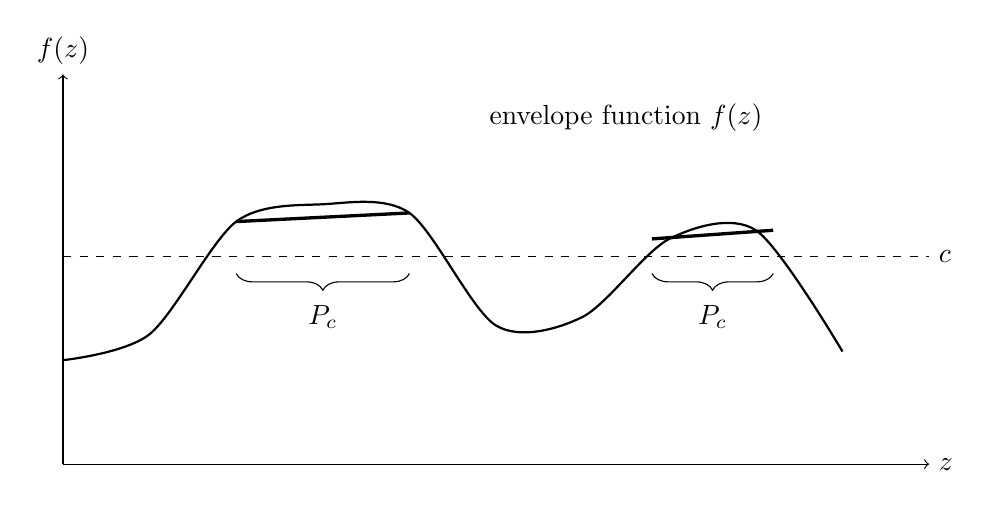
\begin{tikzpicture}[scale=1.1]

% Axes
        \draw[->] (0,0) -- (10,0) node[right] {$z$};
        \draw[->] (0,0) -- (0,4.5) node[above] {$f(z)$};

% Envelope function f(z)
        \draw[thick, smooth]
        plot coordinates {
          (0,1.2)
          (1,1.5)
          (2,2.8)
          (3,3.0)
          (4,2.9)
          (5,1.6)
          (6,1.7)
          (7,2.6)
          (8,2.7)
          (9,1.3)
        };

% Threshold
        \draw[dashed] (0,2.4) -- (10,2.4)
        node[right] {$c$};

% Highlight projected intervals
        \draw[very thick] (2.0,2.8) -- (4.0,2.9);
        \draw[very thick] (6.8,2.6) -- (8.2,2.7);

% Braces for Pc
        \draw[decorate,decoration={brace,mirror,amplitude=6pt}]
        (2.0,2.2) -- (4.0,2.2)
        node[midway,below=8pt] {$P_c$};

        \draw[decorate,decoration={brace,mirror,amplitude=6pt}]
        (6.8,2.2) -- (8.2,2.2)
        node[midway,below=8pt] {$P_c$};

% Labels
        \node at (6.5,4.0) {envelope function $f(z)$};

      \end{tikzpicture}
      \caption{Projection-induced apparent discontinuities.
      The envelope function $f(z)=\max_{x,y}\phi(x,y,z)$ is continuous, but the projected set
        $P_c=\{z\mid f(z)\ge c\}$ consists of disjoint intervals.
        The apparent fragmentation results from thresholding and does not reflect any
        discontinuity of the underlying scalar field $\phi$.}
      \label{fig:levelset_projection}
    \end{figure}

    Importantly, the apparent disjointness of $P_c$ does not imply any discontinuity of the underlying
    field $\phi$.
    Rather, it arises from the fact that only regions exceeding the chosen threshold $c$ are retained.
    The fragmentation is therefore a projection effect induced by thresholding.

  \subsubsection{Envelope Function and Threshold Visibility}

    Define the envelope function
    \begin{equation}
      f(z) = \max_{x,y} \phi(x,y,z).
    \end{equation}

    The set $P_c$ can then be written equivalently as
    \begin{equation}
      P_c = \{ z \in \mathbb{R} \mid f(z) \ge c \}.
    \end{equation}

    The function $f(z)$ is uniquely determined by $\phi$ and provides a global one-dimensional
    summary of the field's maximal amplitude along each slice of constant $z$.
    While the full three-dimensional structure of $\phi$ cannot be reconstructed from $P_c$ alone,
    the envelope function $f(z)$ encodes the emergence and disappearance of visible components as the
    threshold $c$ is varied.

    In this sense, threshold-based visualizations reveal sections of a continuous structure rather
    than discrete or independent objects.

  \subsubsection{Non-Uniqueness of Inverse Reconstruction}

    Given a projected set $P_c$ or a collection of disjoint level-set components, the inverse problem
    of reconstructing $\phi$ is not uniquely solvable.
    Multiple continuous scalar fields may share identical level sets at a given threshold.

    Additional assumptions---such as symmetry, minimal curvature, smoothness, or governing differential
    equations---are required to select a preferred reconstruction.
    The present result therefore establishes a structural constraint rather than a unique inversion.

  \subsubsection{Summary}

    Level-set visualizations of continuous scalar fields generically produce apparently disjoint
    structures when projected or thresholded.
    These structures should be understood as emergent sections of an underlying continuous field.
    The mathematical origin of this effect is independent of any specific physical interpretation,
    but it provides a natural geometric framework for understanding disjoint orbital-like patterns
    as manifestations of threshold visibility.

    While this appendix is presented independently of any physical model, the
    results apply directly to situations in which observable structures are
    defined by detection thresholds or projection procedures, as in atomic,
    optical, or imaging contexts.

    These effects are purely geometric and arise generically whenever continuous scalar
    fields are visualized through threshold-based projections (see Fig.~\ref{fig:levelset_projection}).

  \subsection{Emergent Electrodynamics from $\chi$ Dynamics}
  \label{app:emergent-electrodynamics}

  In regimes where the $\chi$ field admits a smooth geometric and weak-gradient
  description, small perturbations around a slowly varying background obey an
  effective wave equation derived from the variational formulation
  (Section~\ref{subsec:variational-formulation}):
  \begin{equation}
    \nabla \cdot
    \left(
      \frac{\nabla \chi}{\sqrt{1 - |\nabla \chi|^2 / c^2}}
    \right)
    - \frac{1}{c^2} \frac{\partial^2 \chi}{\partial t^2}
    =
    \frac{4 \pi G_{\mathrm{eff}}}{c^2} \rho_\chi .
  \end{equation}

  In the weak-field limit, $|\nabla \chi| \ll c$, this equation linearizes to
  \begin{equation}
    \nabla^2 \chi
    - \frac{1}{c^2} \frac{\partial^2 \chi}{\partial t^2}
    =
    4 \pi G_{\mathrm{eff}} \rho_\chi ,
  \end{equation}
  which admits propagating solutions interpreted as radiative disturbances of the
  $\chi$ field.

  \subsubsection*{Emergent Scalar and Vector Potentials}

    Electromagnetic-like degrees of freedom arise from the \emph{geometric structure}
    of $\chi$ perturbations rather than from independent fundamental fields.
    In regions containing charged solitonic excitations, the spatial gradients of
    $\chi$ acquire both longitudinal and transverse components.

    Accordingly, the spatial gradient of $\chi$ may be decomposed (at the effective
    level) into longitudinal and transverse parts:
    \begin{equation}
      \nabla \chi = - \nabla \phi + \mathbf{A}_{\mathrm{T}},
    \end{equation}
    where $\phi$ is an effective scalar potential and $\mathbf{A}_{\mathrm{T}}$ is a
    divergence-free vector field,
    \begin{equation}
      \nabla \cdot \mathbf{A}_{\mathrm{T}} = 0 .
    \end{equation}

    This decomposition should be understood as an effective Helmholtz projection
    induced by the topology of localized $\chi$ excitations, rather than as a
    fundamental split of degrees of freedom.
    The scalar component encodes longitudinal relaxation gradients associated with
    effective charge density, while the transverse component arises from solitonic
    configurations with non-trivial circulation.

  \subsubsection*{Topological Origin of the Vector Potential}

    The transverse component $\mathbf{A}_{\mathrm{T}}$ originates from solitonic
    configurations of $\chi$ characterized by non-vanishing loop integrals
    \begin{equation}
      \oint \nabla \chi \cdot d\mathbf{l} \neq 0 ,
    \end{equation}
    as discussed in Section~\ref{subsec:vortices}.
    Such configurations imply the existence of an effective vector potential whose
    curl is non-zero, while its divergence vanishes identically.

    The vector potential is therefore not an independent dynamical field.
    It is a derived quantity encoding the transverse sector of $\chi$ gradients,
    analogous to vorticity-induced vector fields in fluid dynamics.

  \subsubsection*{Emergent Electromagnetic Fields}

    Within this effective description, the electric and magnetic fields are defined as
    \begin{equation}
      \mathbf{E}
      =
      - \nabla \phi
      - \frac{1}{c} \frac{\partial \mathbf{A}_{\mathrm{T}}}{\partial t},
      \qquad
      \mathbf{B}
      =
      \nabla \times \mathbf{A}_{\mathrm{T}} .
    \end{equation}

    These fields satisfy the Maxwell equations:
    \begin{align}
      \nabla \cdot \mathbf{E}
      &= 4 \pi G_{\mathrm{eff}} \rho_{\mathrm{em}}, \\
      \nabla \times \mathbf{E}
      + \frac{1}{c} \frac{\partial \mathbf{B}}{\partial t}
      &= 0, \\
      \nabla \cdot \mathbf{B}
      &= 0, \\
      \nabla \times \mathbf{B}
      - \frac{1}{c} \frac{\partial \mathbf{E}}{\partial t}
      &=
      \frac{4 \pi G_{\mathrm{eff}}}{c} \mathbf{J}_{\mathrm{em}},
    \end{align}
    where $\rho_{\mathrm{em}}$ and $\mathbf{J}_{\mathrm{em}}$ denote the effective charge
    and current densities associated with solitonic $\chi$ excitations.

  \subsubsection*{Gauge Invariance}

    The decomposition of $\nabla \chi$ into scalar and transverse components is not
    unique.
    A transformation of the form
    \begin{equation}
      \phi \rightarrow \phi - \frac{1}{c} \frac{\partial \Lambda}{\partial t},
      \qquad
      \mathbf{A}_{\mathrm{T}} \rightarrow \mathbf{A}_{\mathrm{T}} + \nabla \Lambda ,
    \end{equation}
    leaves the observable fields $\mathbf{E}$ and $\mathbf{B}$ invariant.

    This emergent $U(1)$ gauge symmetry reflects the relational nature of $\chi$:
    only differences of gradients have operational meaning, while the absolute
    potential is unobservable
    (Section~\ref{subsec:relational-foundation-pointer}).

  \subsubsection*{Interpretational Status}

    The Maxwell-like structure derived here is not fundamental.
    It arises as a universal effective description of transverse $\chi$ perturbations
    in regimes where solitonic topology and weak gradients coexist.
    Electromagnetism therefore appears as a geometric manifestation of the relational
    and topological structure of the $\chi$ field, rather than as an independent
    interaction mediated by elementary gauge fields.

